\chapter{Results and Analysis} 
%Created 21-12-2016 (04-03-2016 first) 
\label{ch:results}
With the program validated, both case 1 and case 2 can be used to examine the behaviour of \ac{TSI}. This is done in a sensitivity analysis and is very useful to determine the limitations and characteristics of this method. In the previous chapter the trajectories from both \ac{TSI} and \ac{RKF} were plotted and it could be seen that the results were very similar to the point where the accuracy of \ac{TSI} was validated. Therefore, in this chapter the performance of \ac{TSI} will be compared to \ac{RKF} to determine any advantages and disadvantages. In order to do this only one variable will be changed every time, which means that from the nominal case only one parameter will be different. This way the effects can be clearly associated with that particular parameter, which provides a solid base of comparison. The nominal values for both the first and second case are provided in \Cref{app:appendixF-nominalCaseInputValues}. It is also important to have the same cut-off point. This can either be a certain altitude, set end time or zero degrees flight-path angle. Usually the set end time is taken as the cut-off criteria to determine the difference in state. Sometimes the altitude is used in cases where it is interesting to see when a certain altitude is reached and under what conditions when a certain parameter is changed. An example was shown in the validation chapter where certain conditions had to be met at a certain altitude. And in some cases it is best to set the zero degrees flight-path angle as a cut-off criteria because either the cut-off time or altitude will never be reached but the effects of a parameter still need to be investigated. This last cut-off criteria is the "fail-safe" for every simulation because this prevents the simulation from going back to the surface and literally crashing the program. In this chapter every section discusses the effect of a different parameter or focusses on one aspect of the simulation. \\

Besides comparing \ac{TSI} to \ac{RKF} it will also be compared to the non-rotational case. The nominal case takes the rotating Mars into account, however it is interesting to see what \ac{TSI} does when the rotation is turned off. For these two cases to be properly compared, again for most parameters, the set end time is the cut-off criteria unless mentioned otherwise.\\

The parameters changed in this sensitivity analysis are: order, error tolerance, launch altitude, launch latitude, launch longitude, flight-path angle and heading angle. A multiple run analysis will also be described where the nominal case is run for a number of times and the CPU time is compared. 


\section{Order}
\label{sec:order}
Mention what I want to discuss in this section.

\subsection{Optimal order}
\label{subsec:optimalOrder}
Show both plots of orders and then talk about the fastest order and explain what you can see. First part of graph is the number of evaluations important and last part is the amount of computations that have to be made because the number of evaluations don't change any more.

Graphs needed:

- CPU time vs order case 1 and case 2

% \begin{figure}[!ht]
%\centering
%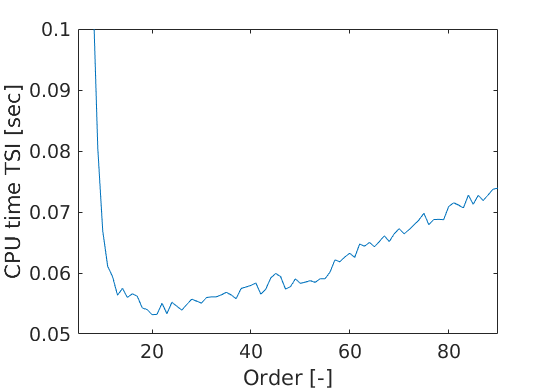
\includegraphics[width=0.7\textwidth]{figures/results/Order/orderVsCPUcase1IncludingLiveDataCollection.png}
%\caption{Order versus CPU time case 1 including live data collection.}
%\label{fig:orderVsCPUcase1IncludingLiveDataCollection}
%\end{figure}

%\begin{figure}
%\centering
%\subfloat[]{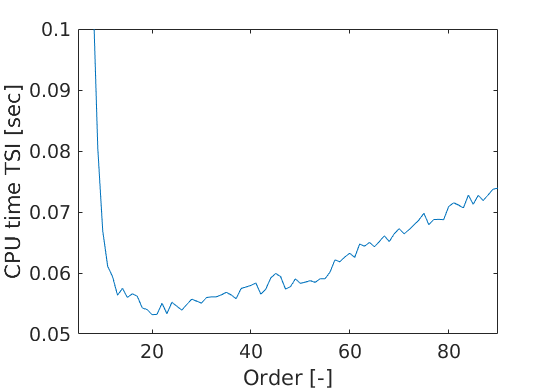
\includegraphics[width=3.1in]{figures/results/Order/orderVsCPUcase1IncludingLiveDataCollection.png}\label{subfig:orderVsCPUcase1IncludingLiveDataCollection}} 
%\subfloat[]{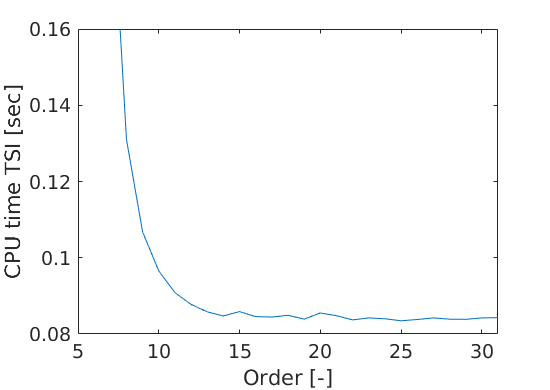
\includegraphics[width=3.1in]{figures/results/Order/orderVsCPUcase2IncludingLiveDataCollection.png}\label{subfig:orderVsCPUcase2IncludingLiveDataCollection}}
%\caption{Order versus CPU time including live data collection \protect\subref{subfig:orderVsCPUcase1IncludingLiveDataCollection} case 1 \protect\subref{subfig:orderVsCPUcase2IncludingLiveDataCollection} case 2 } 
%\label{fig:orderVsCPUcase1IncludingLiveDataCollection} 
%\end{figure} 
%
%\begin{figure}
%\centering
%\subfloat[]{\includegraphics[width=3.1in]{figures/results/Order/orderVsCPUcase1NoDataCollection.png}\label{subfig:orderVsCPUcase1NoDataCollection}} 
%\subfloat[]{\includegraphics[width=3.1in]{figures/results/Order/orderVsCPUcase2NoDataCollection.png}\label{subfig:orderVsCPUcase2NoDataCollection}}
%\caption{Order versus CPU time without live data collection \protect\subref{subfig:orderVsCPUcase1NoDataCollection} case 1 \protect\subref{subfig:orderVsCPUcase2NoDataCollection} case 2 } 
%\label{fig:orderVsCPUcase1NoDataCollection} 
%\end{figure} 

\begin{figure}
\centering
\subfloat[]{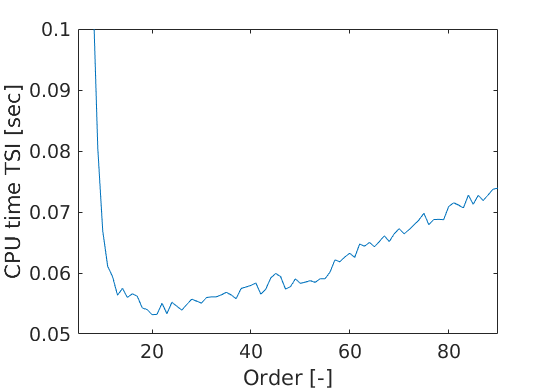
\includegraphics[width=3.1in]{figures/results/Order/orderVsCPUcase1IncludingLiveDataCollection.png}\label{subfig:orderVsCPUcase1IncludingLiveDataCollection}} 
\subfloat[]{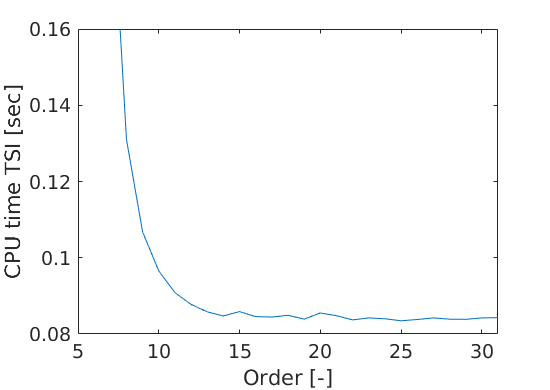
\includegraphics[width=3.1in]{figures/results/Order/orderVsCPUcase2IncludingLiveDataCollection.png} \label{subfig:orderVsCPUcase2IncludingLiveDataCollection}}\\
 
\subfloat[]{\includegraphics[width=3.1in]{figures/results/Order/orderVsCPUcase1NoDataCollection.png}\label{subfig:orderVsCPUcase1NoDataCollection}} 
\subfloat[]{\includegraphics[width=3.1in]{figures/results/Order/orderVsCPUcase2NoDataCollection.png}\label{subfig:orderVsCPUcase2NoDataCollection}}
\caption{Order versus CPU time \protect\subref{subfig:orderVsCPUcase1IncludingLiveDataCollection} case 1 including live data collection, \protect\subref{subfig:orderVsCPUcase2IncludingLiveDataCollection} case 2 including live data collection, \protect\subref{subfig:orderVsCPUcase1NoDataCollection} case 1 without live data collection, \protect\subref{subfig:orderVsCPUcase2NoDataCollection} case 2 without live data collection } 
\label{fig:orderVsCPUcase1IncludingLiveDataCollection} 
\end{figure} 



\subsection{Comparison with non-rotating Mars}
\label{subsec:orderCompNotRot}

Explain what you can see in the graph and why that is probably the case.

Graphs needed:

- CPU time vs order case 1 combined \\
- CPU time vs order case 2 combined \\


- RKF difference in end state before circularisation combined case 1 \\ 
- RKF difference in end state before circularisation combined case 2 \\
- Consecutive difference in end state before cicularisation combined case 1 \\
- Consecutive difference in end state before cicularisation combined case 2 \\
- Nominal case difference in end state before circularisation combined case 1 \\
- Nominal case difference in end state before circularisation combined case 2 \\

Tables needed:

- Zoom in numbers around Order 20 to prove it is the fastest \\

\begin{figure}
\centering
\subfloat[]{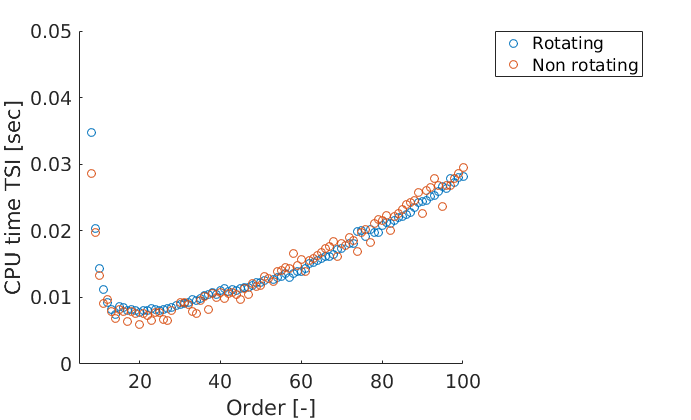
\includegraphics[width=3.1in]{figures/results/Order/orderVsCPUcase1combined.png}\label{subfig:orderVsCPUcase1combined}} 
\subfloat[]{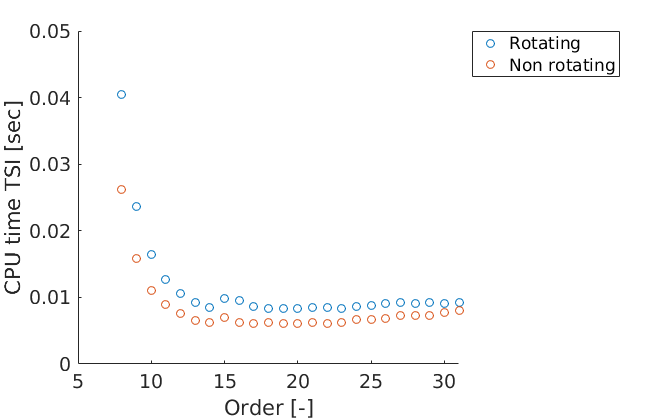
\includegraphics[width=3.1in]{figures/results/Order/orderVsCPUcase2combined.png}\label{subfig:orderVsCPUcase2combined}}
\caption{Order versus CPU time for rotating and non-rotating Mars \protect\subref{subfig:orderVsCPUcase1combined} case 1,  \protect\subref{subfig:orderVsCPUcase2combined} case 2 } 
\label{fig:orderVsCPUcase1combined} 
\end{figure} 

\begin{figure}
\centering
\subfloat[]{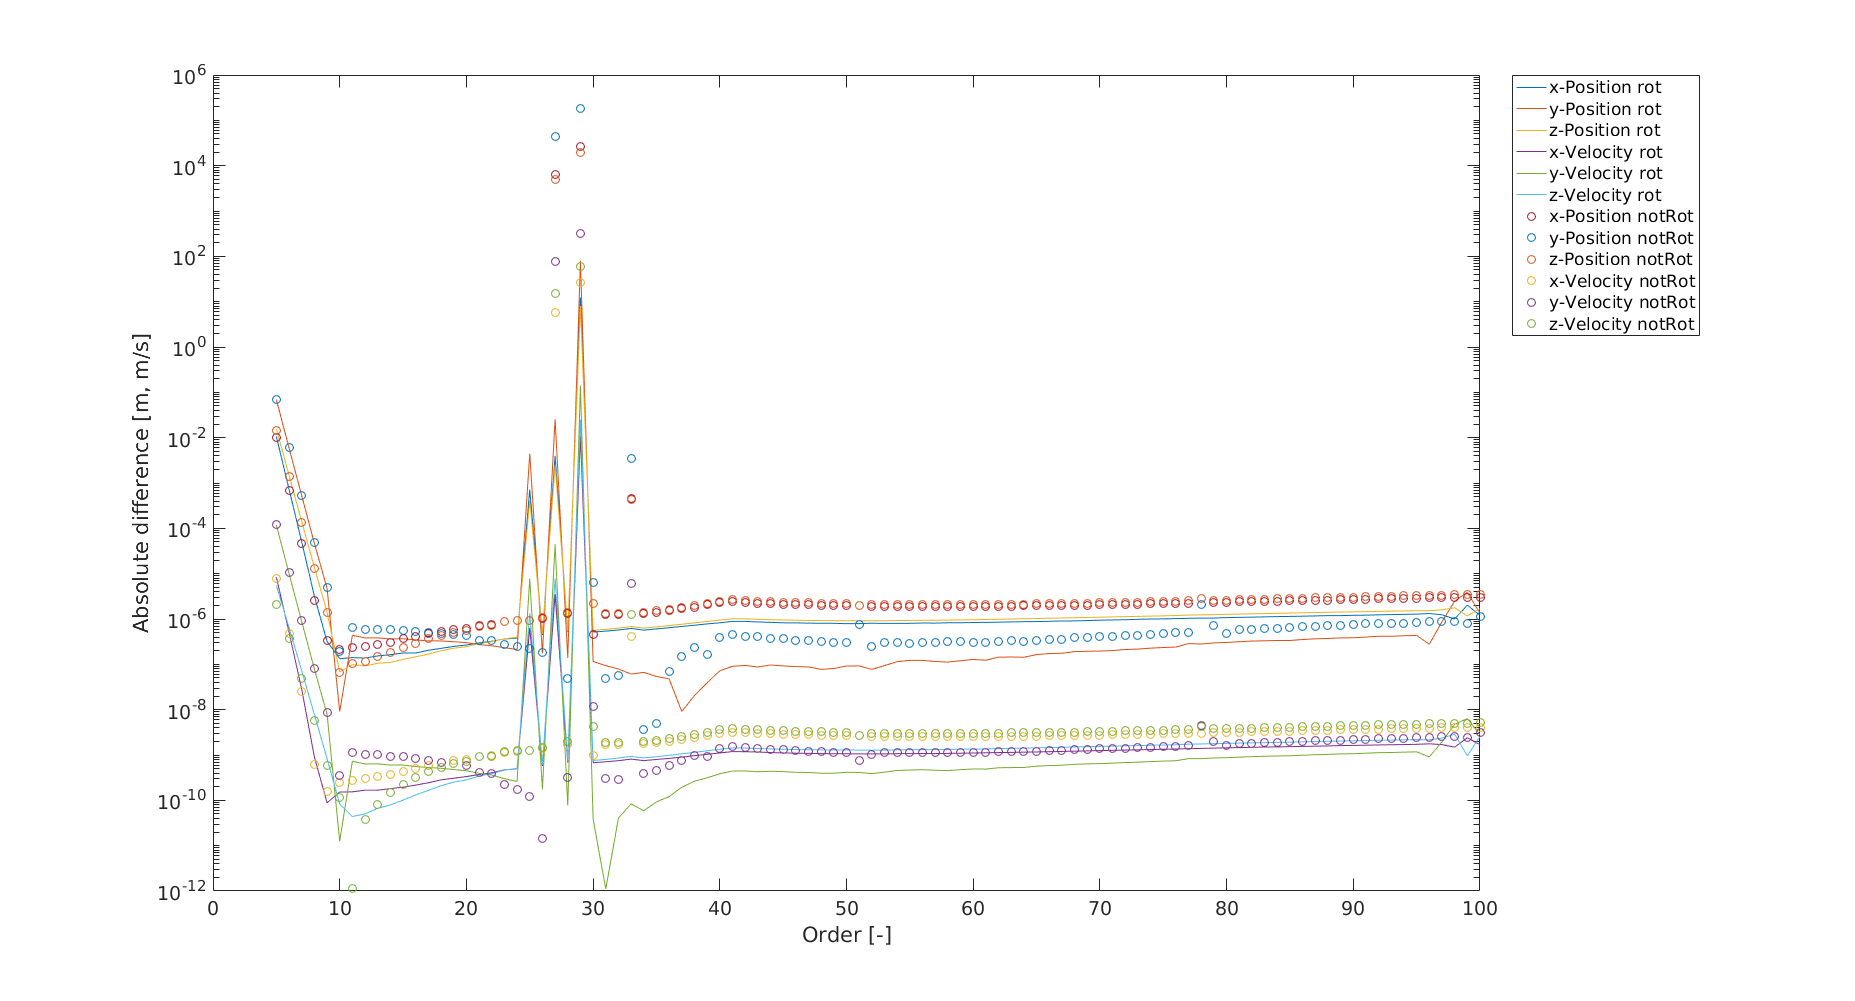
\includegraphics[width=1.2\textwidth]{figures/results/Order/orderVsRKFAbsoluteDifferenceCase1combined.png}\label{subfig:orderVsRKFAbsoluteDifferenceCase1combined}}\\
 
\subfloat[]{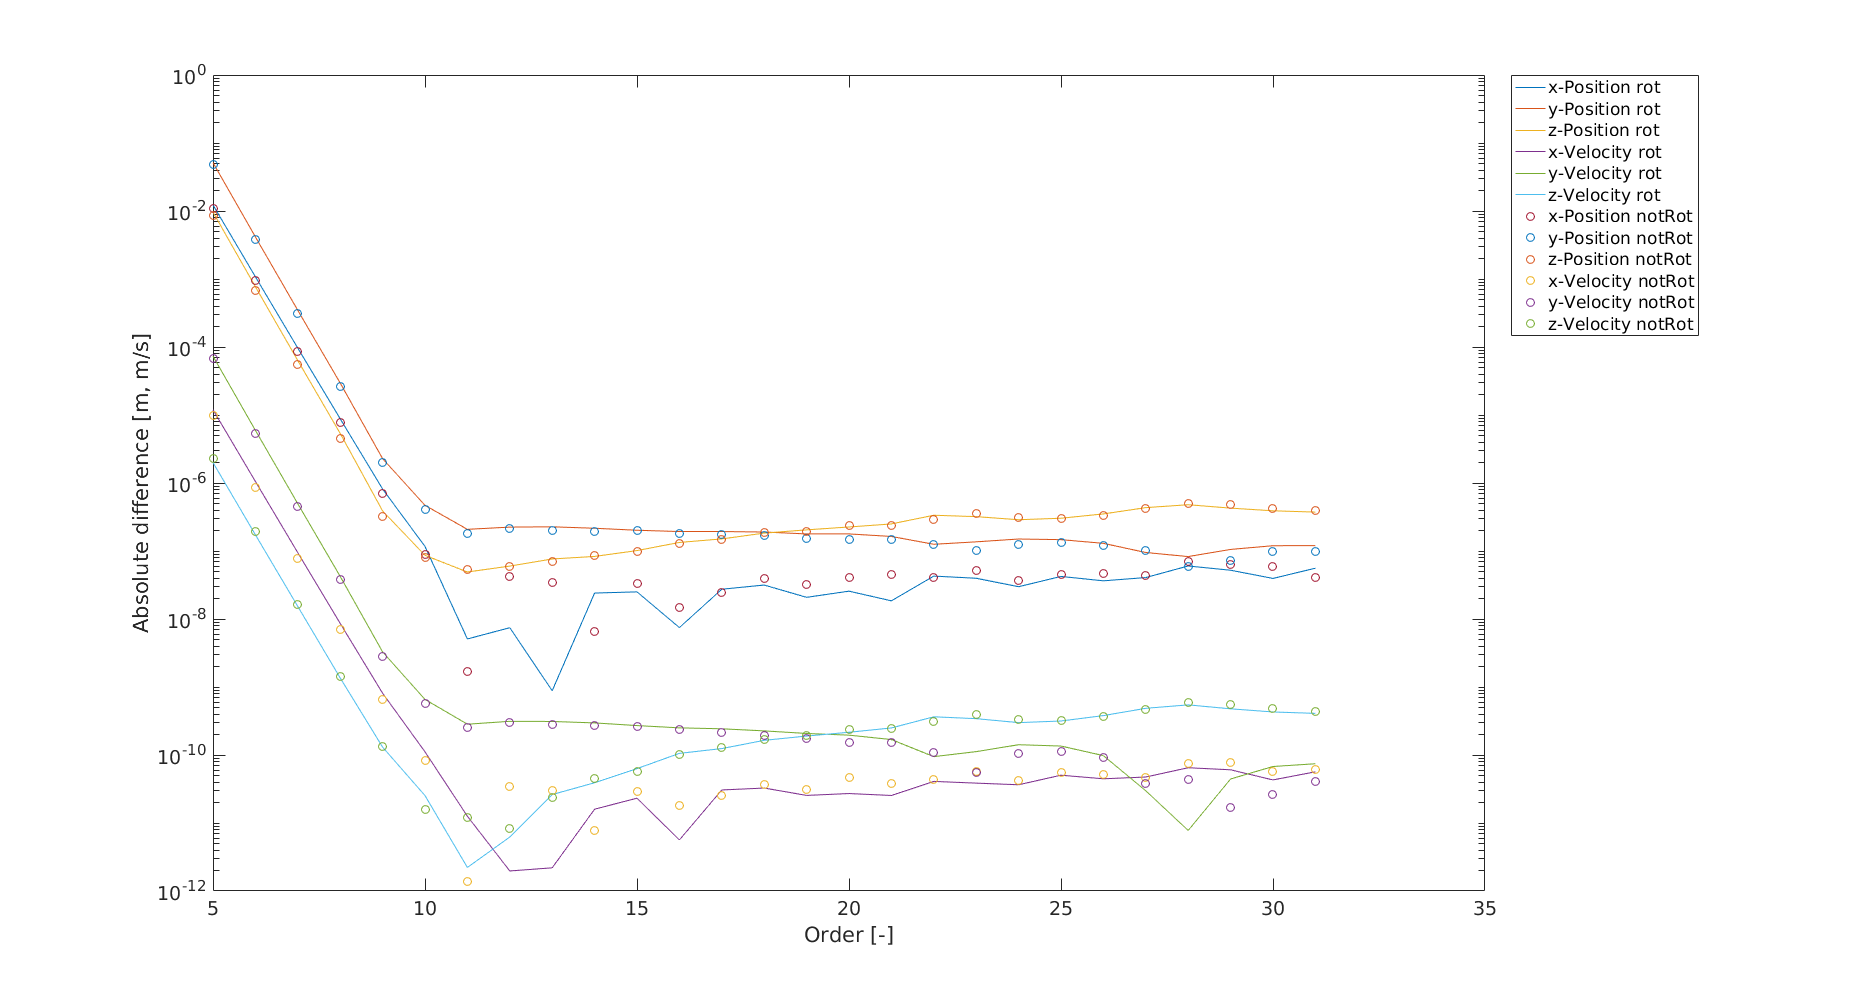
\includegraphics[width=1.2\textwidth]{figures/results/Order/orderVsRKFAbsoluteDifferenceCase2combined.png}\label{subfig:orderVsRKFAbsoluteDifferenceCase2combined}}
\caption{Difference with respect to \ac{RKF} case for rotating and non-rotating Mars \protect\subref{subfig:orderVsRKFAbsoluteDifferenceCase1combined} case 1,  \protect\subref{subfig:orderVsRKFAbsoluteDifferenceCase2combined} case 2 } 
\label{fig:orderVsRKFAbsoluteDifferenceCase1combined} 
\end{figure}


\section{Error tolerance}
\label{sec:errorTolerance}
Mention what I want to discuss in this section.


\subsection{Comparison with \ac{RKF78}}
\label{subsec:errorToleranceCompRKF}

Show the faster convergence of end state before circularisation.
Compare the number of function evaluations and explain why you should look at the function evaluations in such a manner. So explain that RKF does 13 function evaluations per step and TSI only does one.

Graphs needed:

- Consecutive difference graphs RKF and TSI combined for case 1 \\
- Consecutive difference graphs RKF and TSI combined for case 2 \\
- Nominal case difference in end state before circularisation RKF and TSI combined case 1 \\
- Nominal case difference in end state before circularisation RKF and TSI combined case 2 \\

\begin{figure}
\centering
\subfloat[]{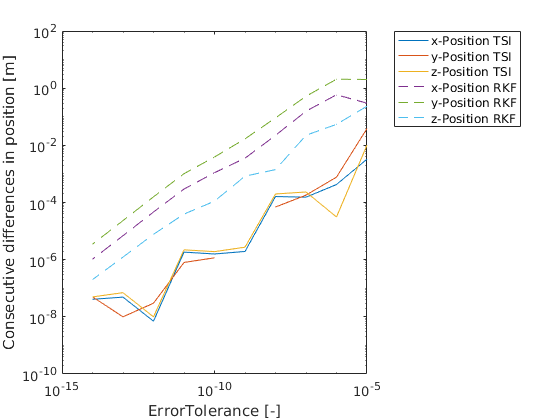
\includegraphics[width=3.1in]{figures/results/errorTolerance/errorToleranceVsConsecutiveDifferenceCase1RKFTSIpositionSmall.png}\label{subfig:errorToleranceVsConsecutiveDifferenceCase1RKFTSIpositionSmall}} 
\subfloat[]{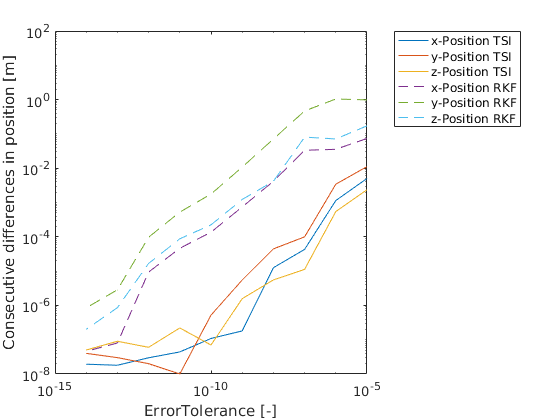
\includegraphics[width=3.1in]{figures/results/errorTolerance/errorToleranceVsConsecutiveDifferenceCase2RKFTSIpositionSmall.png} \label{subfig:errorToleranceVsConsecutiveDifferenceCase2RKFTSIpositionSmall}}\\
 
\subfloat[]{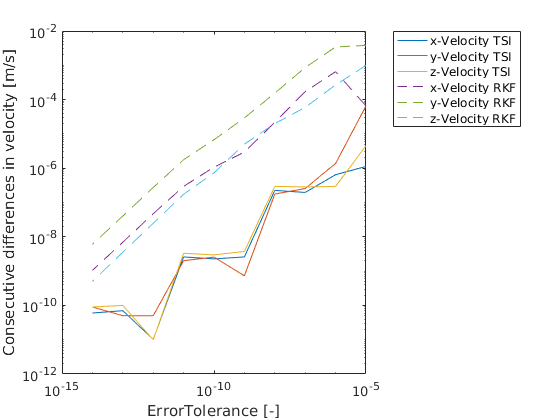
\includegraphics[width=3.1in]{figures/results/errorTolerance/errorToleranceVsConsecutiveDifferenceCase1RKFTSIvelocitySmall.png}\label{subfig:errorToleranceVsConsecutiveDifferenceCase1RKFTSIvelocitySmall}} 
\subfloat[]{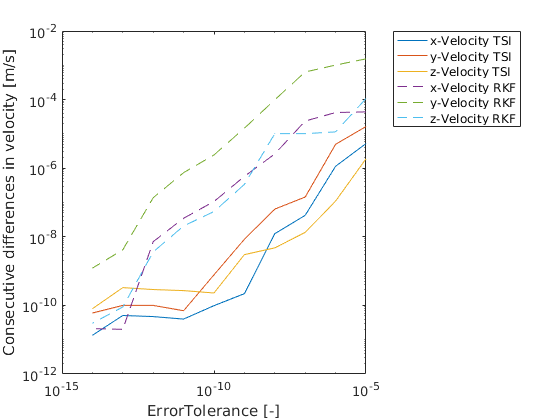
\includegraphics[width=3.1in]{figures/results/errorTolerance/errorToleranceVsConsecutiveDifferenceCase2RKFTSIvelocitySmall.png}\label{subfig:errorToleranceVsConsecutiveDifferenceCase2RKFTSIvelocitySmall}}
\caption{Error tolerance versus consecutive difference between end states before circularisation for \ac{TSI} and \ac{RKF} \protect\subref{subfig:errorToleranceVsConsecutiveDifferenceCase1RKFTSIpositionSmall} case 1 position, \protect\subref{subfig:errorToleranceVsConsecutiveDifferenceCase2RKFTSIpositionSmall} case 2 position, \protect\subref{subfig:errorToleranceVsConsecutiveDifferenceCase1RKFTSIvelocitySmall} case 1 velocity, \protect\subref{subfig:errorToleranceVsConsecutiveDifferenceCase2RKFTSIvelocitySmall} case 2 velocity } 
\label{fig:errorToleranceVsConsecutiveDifferenceCase1RKFTSIpositionSmall} 
\end{figure} 


\begin{figure}
\centering
\subfloat[]{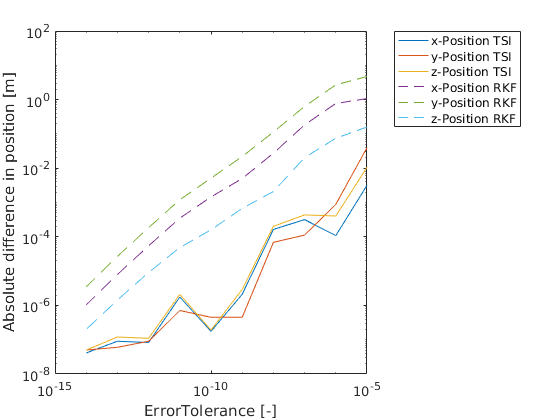
\includegraphics[width=3.1in]{figures/results/errorTolerance/errorToleranceVsNominalAbsoluteDifferenceCase1RKFTSIpositionSmall.png}\label{subfig:errorToleranceVsNominalAbsoluteDifferenceCase1RKFTSIpositionSmall}} 
\subfloat[]{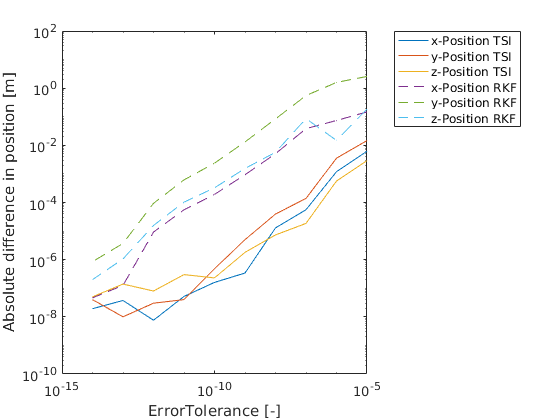
\includegraphics[width=3.1in]{figures/results/errorTolerance/errorToleranceVsNominalAbsoluteDifferenceCase2RKFTSIpositionSmall.png} \label{subfig:errorToleranceVsNominalAbsoluteDifferenceCase2RKFTSIpositionSmall}}\\
 
\subfloat[]{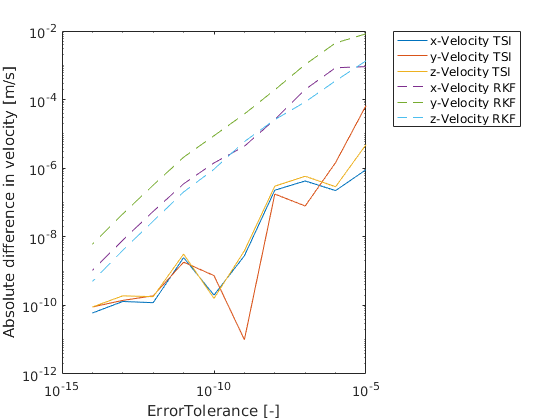
\includegraphics[width=3.1in]{figures/results/errorTolerance/errorToleranceVsNominalAbsoluteDifferenceCase1RKFTSIvelocitySmall.png}\label{subfig:errorToleranceVsNominalAbsoluteDifferenceCase1RKFTSIvelocitySmall}} 
\subfloat[]{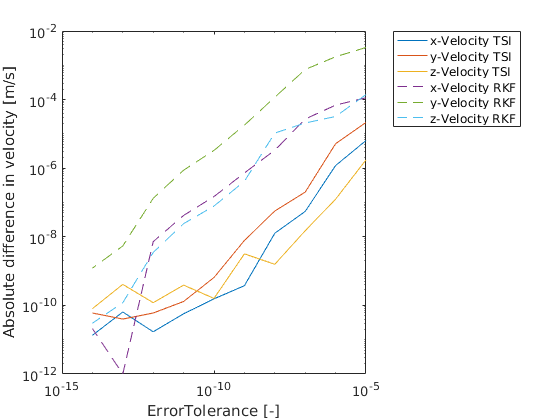
\includegraphics[width=3.1in]{figures/results/errorTolerance/errorToleranceVsNominalAbsoluteDifferenceCase2RKFTSIvelocitySmall.png}\label{subfig:errorToleranceVsNominalAbsoluteDifferenceCase2RKFTSIvelocitySmall}}
\caption{Error tolerance versus nominal absolute difference between end states before circularisation for \ac{TSI} and \ac{RKF} \protect\subref{subfig:errorToleranceVsNominalAbsoluteDifferenceCase1RKFTSIpositionSmall} case 1 position, \protect\subref{subfig:errorToleranceVsNominalAbsoluteDifferenceCase2RKFTSIpositionSmall} case 2 position, \protect\subref{subfig:errorToleranceVsNominalAbsoluteDifferenceCase1RKFTSIvelocitySmall} case 1 velocity, \protect\subref{subfig:errorToleranceVsNominalAbsoluteDifferenceCase2RKFTSIvelocitySmall} case 2 velocity } 
\label{fig:errorToleranceVsNominalAbsoluteDifferenceCase1RKFTSIpositionSmall} 
\end{figure} 

Tables needed:

- Either accuracy of separate coordinates or simply radius in metres \\
- Either accuracy of separate velocities or simply ground velocity in metres/second \\


\subsection{Comparison with non-rotating Mars}
\label{subsec:errorToleranceCompNotRot}
Compare the rotating case with the non-rotating case and see if the convergence speed is different. 

Graphs needed: 

- CPU time vs error tolerance case 1 combined \\
- CPU time vs error tolerance case 2 combined \\
- Consecutive difference in end state before circularisation combined for case 1 \\
- Consecutive difference in end state before circularisation combined for case 2 \\
- Nominal case difference in end state before circularisation combined for case 1 \\
- Nominal case difference in end state before circularisation combined for case 2 \\

\begin{figure}
\centering
\subfloat[]{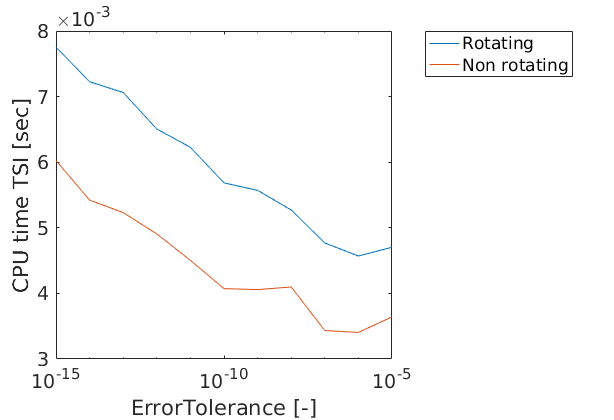
\includegraphics[width=3.1in]{figures/results/errorTolerance/errorToleranceVsCPUcase1combined.png}\label{subfig:errorToleranceVsCPUcase1combined}} 
\subfloat[]{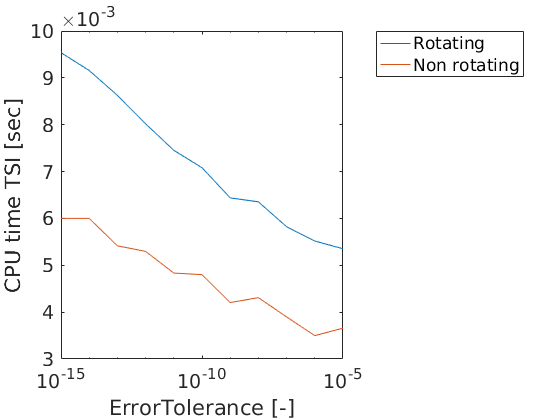
\includegraphics[width=3.1in]{figures/results/errorTolerance/errorToleranceVsCPUcase2combined.png}\label{subfig:errorToleranceVsCPUcase2combined}}
\caption{Error tolerance versus CPU time for rotating and non-rotating Mars \protect\subref{subfig:errorToleranceVsCPUcase1combined} case 1,  \protect\subref{subfig:errorToleranceVsCPUcase2combined} case 2 } 
\label{fig:orderVsCPUcase1combined} 
\end{figure} 

\begin{figure}
\centering
\subfloat[]{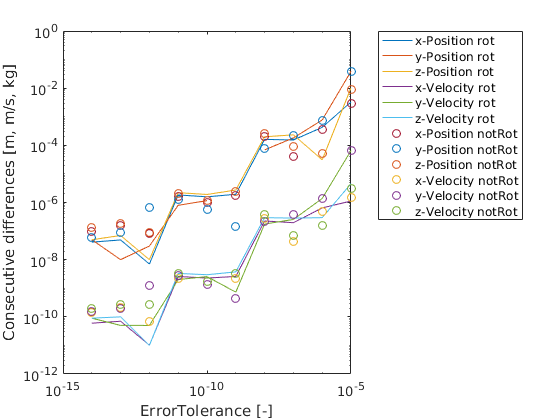
\includegraphics[width=3.1in]{figures/results/errorTolerance/errorToleranceVsConsecutiveDifferenceCase1combinedSmall.png}\label{subfig:errorToleranceVsConsecutiveDifferenceCase1combinedSmall}} 
\subfloat[]{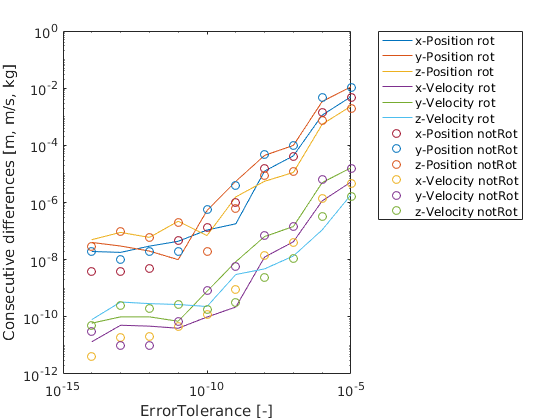
\includegraphics[width=3.1in]{figures/results/errorTolerance/errorToleranceVsConsecutiveDifferenceCase2combinedSmall.png}\label{subfig:errorToleranceVsConsecutiveDifferenceCase2combinedSmall}}
\caption{Error tolerance versus consecutive difference for rotating and non-rotating Mars \protect\subref{subfig:errorToleranceVsConsecutiveDifferenceCase1combinedSmall} case 1,  \protect\subref{subfig:errorToleranceVsConsecutiveDifferenceCase2combinedSmall} case 2 } 
\label{fig:errorToleranceVsConsecutiveDifferenceCase1combinedSmall} 
\end{figure} 

\begin{figure}
\centering
\subfloat[]{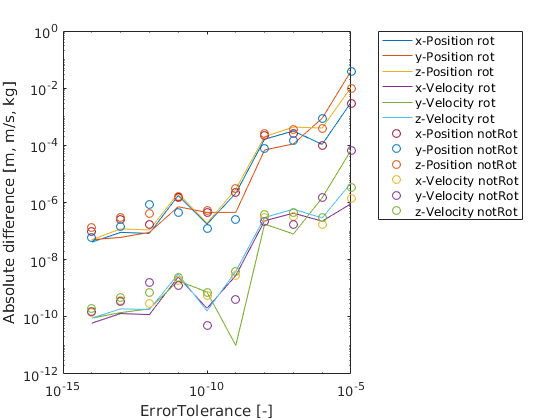
\includegraphics[width=3.1in]{figures/results/errorTolerance/errorToleranceVsNominalAbsoluteDifferenceCase1combinedSmall.png}\label{subfig:errorToleranceVsNominalAbsoluteDifferenceCase1combinedSmall}} 
\subfloat[]{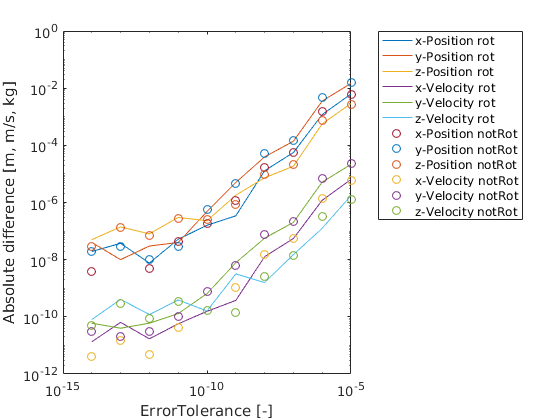
\includegraphics[width=3.1in]{figures/results/errorTolerance/errorToleranceVsNominalAbsoluteDifferenceCase2combinedSmall.png}\label{subfig:errorToleranceVsNominalAbsoluteDifferenceCase2combinedSmall}}
\caption{Error tolerance versus nominal absolute difference for rotating and non-rotating Mars \protect\subref{subfig:errorToleranceVsNominalAbsoluteDifferenceCase1combinedSmall} case 1,  \protect\subref{subfig:errorToleranceVsNominalAbsoluteDifferenceCase2combinedSmall} case 2 } 
\label{fig:errorToleranceVsNominalAbsoluteDifferenceCase1combinedSmall} 
\end{figure} 


Tables needed:

- Either accuracy of separate coordinates or simply radius in metres \\
- Either accuracy of separate velocities or simply ground velocity in metres/second \\


\section{Multiple runs}
\label{sec:multipleRuns}

Mention what I want to discuss in this section.

\subsection{Comparison with \ac{RKF78}}
\label{subsec:timeCompRKF}
Show that RKF is faster than TSI at the moment. Explain why this might be the case and why this was unexpected. Also explain the outliers and different patterns visible. 

Graphs needed:

- Combined RKF and TSI 5000 run plot for case 1 \\
- Combined RKF and TSI 5000 run plot for case 2 \\

\begin{figure}
\centering
\subfloat[]{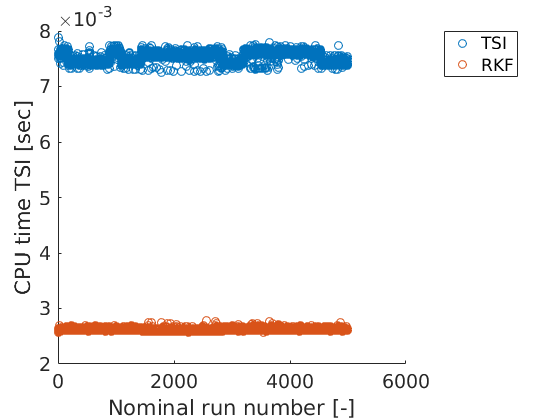
\includegraphics[width=3.1in]{figures/results/multiRun/multiRunVsCPUcase1RKFTSIsmall.png}\label{subfig:multiRunVsCPUcase1RKFTSIsmall}} 
\subfloat[]{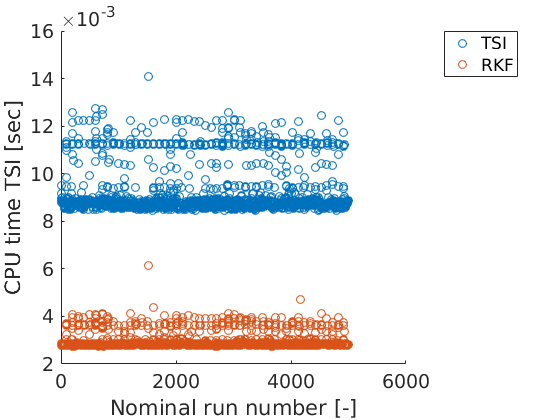
\includegraphics[width=3.1in]{figures/results/multiRun/multiRunVsCPUcase2RKFTSIsmall.png}\label{subfig:multiRunVsCPUcase2RKFTSIsmall}}
\caption{Nominal runs versus CPU time comparison between \ac{RKF} and \ac{TSI} \protect\subref{subfig:multiRunVsCPUcase1RKFTSIsmall} case 1,  \protect\subref{subfig:multiRunVsCPUcase2RKFTSIsmall} case 2 } 
\label{fig:multiRunVsCPUcase1RKFTSIsmall} 
\end{figure} 

Table needed:

- Lowest CPU time for both RKF and TSI \\



\subsection{Comparison with non-rotating Mars}
\label{subsec:timeCompNotRot}
Show the notable difference between the rotating and non-rotating case. Explain why this is the case.

Graphs needed:

- Combined 5000 run plot rot and not rot for case 1 \\
- Combined 5000 run plot rot and not rot for case 2 \\


\begin{figure}
\centering
\subfloat[]{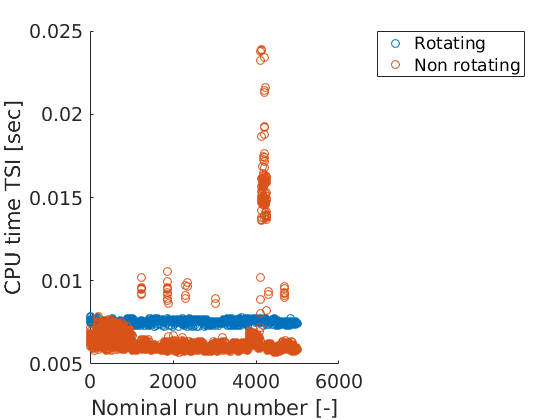
\includegraphics[width=3.1in]{figures/results/multiRun/multiRunVsCPUcase1combinedSmall.png}\label{subfig:multiRunVsCPUcase1combinedSmall}} 
\subfloat[]{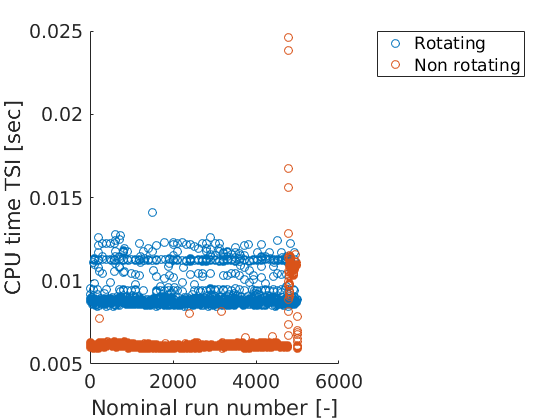
\includegraphics[width=3.1in]{figures/results/multiRun/multiRunVsCPUcase2combinedSmall.png}\label{subfig:multiRunVsCPUcase2combinedSmall}}
\caption{Nominal runs versus CPU time for rotating and non-rotating Mars \protect\subref{subfig:multiRunVsCPUcase1combinedSmall} case 1,  \protect\subref{subfig:multiRunVsCPUcase2combinedSmall} case 2 } 
\label{fig:multiRunVsCPUcase1combinedSmall} 
\end{figure} 



\section{Launch altitude}
\label{sec:launchAltitude}

Only comparison with non-rotating Mars and simply look at the different altitudes and the effects

Graphs needed:

- CPU time vs order case 1 combined \\
- CPU time vs order case 2 combined \\
- Circularisation propellant mass comb case 1 (if different end conditions were used then once with comb and once just the case 1) \\
- Circularisation propellant mass comb case 2 (if different end conditions were used then once with comb and once just the case 2) \\
- Consecutive differences end state before circularisation comb case 1 \\
- Consecutive differences end state before circularisation comb case 2 \\
- Differences nominal case end state before circularisation comb case 1 \\
- Differences nominal case end state before circularisation comb case 2 \\


Tables needed:

- Radius and difference with nominal case in m case 1 \\
- Radius and difference with nominal case in m case 2 \\
- Ground velocity and difference with nominal case in m case 1 \\
- Ground velocity and difference with nominal case in m case 2 \\





\section{Launch latitude}
\label{sec:launchLatitude}

Only comparison with non-rotating Mars and simply look at the different latitudes and the effects
Show for both cases the differences in x,y and z position and velocity. Do case 1 and 2 look similar? Why do the graphs look a certain way?

Graphs needed:

- CPU time vs order case 1 combined (if not random) \\
- CPU time vs order case 2 combined (if not random) \\
- All position graphs case 1 \\
- All position graphs case 2 \\
- All velocity graphs case 1 \\
- All velocity graphs case 2 \\

- Circularisation propellant mass comb case 1 (if different end conditions were used then once with comb and once just the case 1) \\
- Circularisation propellant mass comb case 2 (if different end conditions were used then once with comb and once just the case 2) \\
- Consecutive differences end state before circularisation comb case 1 \\
- Consecutive differences end state before circularisation comb case 2 \\
- Differences nominal case end state before circularisation comb case 1 \\
- Differences nominal case end state before circularisation comb case 2 \\


Tables needed:

- Radius and difference with nominal case in m case 1 \\
- Radius and difference with nominal case in m case 2 \\
- Ground velocity and difference with nominal case in m case 1 \\
- Ground velocity and difference with nominal case in m case 2 \\
 


\section{Launch longitude}
\label{sec:launchLongitude}

Only comparison with non-rotating Mars and simply look at the different longitudes and the effects
Show for both cases the differences in x,y and z position and velocity. Do case 1 and 2 look similar? Why do the graphs look a certain way?

Graphs needed:

- CPU time vs order case 1 combined (if not random) \\
- CPU time vs order case 2 combined (if not random) \\
- All position graphs case 1 \\
- All position graphs case 2 \\
- All velocity graphs case 1 \\
- All velocity graphs case 2 \\

- Circularisation propellant mass comb case 1 (if different end conditions were used then once with comb and once just the case 1) \\
- Circularisation propellant mass comb case 2 (if different end conditions were used then once with comb and once just the case 2) \\
- Consecutive differences end state before circularisation comb case 1 \\
- Consecutive differences end state before circularisation comb case 2 \\
- Differences nominal case end state before circularisation comb case 1 \\
- Differences nominal case end state before circularisation comb case 2 \\



\section{Flight-path angle}
\label{sec:flightPathAngle}

Only comparison with non-rotating Mars and simply look at the different Flight-path angles and the effects
Show for both cases the differences in x,y and z position and velocity. Do case 1 and 2 look similar? Why do the graphs look a certain way?
Explain why only a few runs could be done because of the huge initial effect that the FPA has because of the low velocity in the beginning.

Graphs needed:

- CPU time vs order case 1 combined (if not random) \\
- CPU time vs order case 2 combined (if not random) \\
- All position graphs case 1 \\
- All position graphs case 2 \\
- All velocity graphs case 1 \\
- All velocity graphs case 2 \\

- Circularisation propellant mass comb case 1 (if different end conditions were used then once with comb and once just the case 1) \\
- Circularisation propellant mass comb case 2 (if different end conditions were used then once with comb and once just the case 2) \\
- Consecutive differences end state before circularisation comb case 1 \\
- Consecutive differences end state before circularisation comb case 2 \\
- Differences nominal case end state before circularisation comb case 1 \\
- Differences nominal case end state before circularisation comb case 2 \\


Tables needed:

- Radius and difference with nominal case in m case 1 \\
- Radius and difference with nominal case in m case 2 \\
- Ground velocity and difference with nominal case in m case 1 \\
- Ground velocity and difference with nominal case in m case 2 \\

\section{Heading angle}
\label{sec:headingAngle}

Only comparison with non-rotating Mars and simply look at the different heading angles and the effects
Show for both cases the differences in x,y and z position and velocity. Do case 1 and 2 look similar? Why do the graphs look a certain way?

Graphs needed:

- CPU time vs order case 1 combined (if not random) \\
- CPU time vs order case 2 combined (if not random) \\
- All position graphs case 1 \\
- All position graphs case 2 \\
- All velocity graphs case 1 \\
- All velocity graphs case 2 \\

- Circularisation propellant mass comb case 1 (if different end conditions were used then once with comb and once just the case 1) \\
- Circularisation propellant mass comb case 2 (if different end conditions were used then once with comb and once just the case 2) \\
- Consecutive differences end state before circularisation comb case 1 \\
- Consecutive differences end state before circularisation comb case 2 \\
- Differences nominal case end state before circularisation comb case 1 \\
- Differences nominal case end state before circularisation comb case 2 \\


Tables needed:

- Radius and difference with nominal case in m case 1 \\
- Radius and difference with nominal case in m case 2 \\
- Ground velocity and difference with nominal case in m case 1 \\
- Ground velocity and difference with nominal case in m case 2 \\
